% Indicate the main file. Must go at the beginning of the file.
% !TEX root = ../main.tex

%%%%%%%%%%%%%%%%%%%%%%%%%%%%%%%%%%%%%%%%%%%%%%%%%%%%%%%%%%%%%%%%%%%%%%%%%%%%%%%%
% 02_methods
%%%%%%%%%%%%%%%%%%%%%%%%%%%%%%%%%%%%%%%%%%%%%%%%%%%%%%%%%%%%%%%%%%%%%%%%%%%%%%%%

\section{Methods}
\label{methods}

\subsection{Dataset}%%%%%%%%%%%%%%%%%%%%%%%%%%%%%%%%%%%%%%%%%%%%%%%%%%%%%%%%%%%%

In this study, a preexisting dataset is used -- the InsectSet32 dataset \autocite{faissInsectSet32DatasetAutomatic2022}. 
The dataset includes 335 recordings of 32 insect species, totaling 57 minutes.
About half of the recordings (147) feature nine \textit{Orthoptera} species from a dataset originally compiled by Baudewijn Odé (unpublished). 
The remaining 188 recordings, from 23 \textit{Cicadidae} species, were selected from the Global Cicada Sound 
Collection on Bioacoustica \autocite{bakerBioAcousticaFreeOpen2015}, including recordings 
published in \autocites{bakerGlobalCicadaSound2015}{poppleRevisionMyopsaltaCrucifera2017}\todo{Is this okay?}. 
Speech annotations at the beginning of many recordings led to using the last ten seconds of audio. 
Files with strong noise or multiple species were removed. The number of files per species ranges from 4 to 22, 
with durations from 40 seconds to almost 9 minutes. All files, originally with a sampling rate of at least 44.1 kHz, 
were resampled to 44.1 kHz mono WAV for consistency.
The dataset was already split into training, validation and test sets. There are two .csv files containing
the labels and the filenames of the recordings.

\subsection{Programming Language and Frameworks}%%%%%%%%%%%%%%%%%%%%%%%%%%%%%%%%%
To build and train the deep learning model, the programming language Python was used.
The Frameworks PyTorch\replace{,}{and} Lightning are \replace{very popular}{widely used} and powerful tools for building deep learning models.

\subsection{Deep Learning Model}%%%%%%%%%%%%%%%%%%%%%%%%%%%%%%%%%%%%%%%%%%%%%%%%%

The deep learning model used in this study is a convolutional neural network (CNN) with residual blocks \autocite[ResNet; ][]{heDeepResidualLearning2016}
illustrated in \autoref{fig:model_flow_chart}. It consists of three main parts: An input layer,
a number of stacked residual blocks and an fully connected output layer. The input layer is a convolutional layer with a kernel
size of 1 and and output channels set to the base channels (bc) -- for this experiment it was set to 8.
Note that a convolution with a kernel size of 1 is equivalent to using a fully-connected feed-forward layer.
After the convolutional layer, the input is normed with a batch normalization layer and then passed through
a ReLU activation function. Batch normalization can make the training of neural networks more robust and faster, 
and the ReLU activation introduces non-linearity \autocite{Goodfellow-et-al-201}.
The output is than passed trough a number of residual blocks, where
Residual connections facilitate the training of deep neural networks by enabling smoother flow of gradients 
during backpropagation, i.e., the backward pass performed to compute the model gradients \autocite{Goodfellow-et-al-201}. 
The model is implemented dynamically, so the number of residual blocks can be set as a hyperparameter. Each residual block
consists of two convolutional layers, each followed by a batch normalization layer and a ReLU activation function.
The output channels are doubled with every residual block.
The residual connection is implemented by passing the input trough a separated convolutional layer with a kernel size of 1
and the same number of output channels as the output of the convolutional layers in the residual block to
match dimensions. This output is than added to the output of the transformation in the residual block.
At the end of the residual block, the output is passed trough a max pooling layer to reduce the dimensions.
The max pooling layer is implemented to alter the kernel size with every residual block. For every odd residual block
the kernel size is set to n\_max\_pool -- in this experiment it was set to 3 -- reducing the dimensions by a factor of 3.
For every even residual block the kernel size is set to 1, so the dimensions stay the same. The output of the residual blocks
is passed through a dynamic global average pooling layer, and then passed through a fully-connected feed-forward layer. An additional
convolutional layer with kernel size 1 to match the number of classes. The output was flattened and passed through a 
softmax activation function to get the probabilities for each class as a vector of length 
n\_classes -- in this experiment 32 -- elements between 0 and 1 that sum up to 1.

\subsection{Data Processing}%%%%%%%%%%%%%%%%%%%%%%%%%%%%%%%%%%%%%%%%%%%%%%%%%%%%
A custom Dataloader was implemented, to handle the data processing on the fly
and provide the trainer with then data samples matching the chosen indices.
To implement the dataloader, the PyTorch Dataset and DataLoader classes where used.
For the data processing, the torchaudio and numpy libraries where used.
There is two steps to the data processing: Sampling and Transformation.

\subsubsection{Sampling}%%%%%%%%%%%%%%%%%%%%%%%%%%%%%%%%%%%%%%%%%%%%%%%%%%%%%%%
The audio files are of different lengths and the model was fed with consistent, potentially zero-padded samples for consistency.
Since the smallest files are of a length of around 1 second and the longest file is around
160 seconds, a compromise had to be made. On the one hand, trimming the files to a length of 1 second
would mean very little information being available for the model to learn from. On the other
hand, if the files are sampled for a length of more than a second, the short files would need
to be padded with zeros meaning the file starts with an empty part. This could lead
to the model learning from the length of the empty part and not the actual audio signal, i.e., it would be prone to overfitting.
To avoid this, the audio files where sampled to a random length between 1 and 10 seconds and
then padded with zeros to the fixed length of 10 seconds. To implement this, a custom method
was implemented as shown in \autoref{lst:sampling}.

%==== listing: sampling ====%
\begin{lstlisting}[
    language=Python, 
    caption={Python code for the sampling of the filies}, 
    label={lst:sampling}]
import numpy as np
import torch

def get_random_part_padded(self, waveform: Tensor, samplerate: int) -> Tensor:

    min_len_in_samples = int(self.min_len_in_seconds * samplerate)
    max_len_in_samples = int(self.max_len_in_seconds * samplerate)

    if self.min_len_in_seconds == -1:
        sample_start_index = -max_len_in_samples
        sample_end_index = None

    else:
        part_length = np.random.randint(min_len_in_samples, max_len_in_samples + 1)
        sample_length = waveform.shape[1]
        part_length = min(part_length, sample_length)
        sample_start_index = np.random.randint(0, sample_length - part_length + 1)
        sample_end_index = sample_start_index + part_length

    waveform_part = waveform[:, sample_start_index:sample_end_index]
    actual_part_length = waveform_part.shape[1]
    pad_length = max_len_in_samples - actual_part_length
    waveform_pad = torch.nn.functional.pad(waveform_part, pad=(pad_length, 0, 0, 0))

    return waveform_pad
\end{lstlisting}
%===========================%

\subsubsection{Transformation}%%%%%%%%%%%%%%%%%%%%%%%%%%%%%%%%%%%%%%%%%%%%%%%%%%
Audio signals are rich in information, but also contain spurious information.
One way to condense the the information content of audio data is the transformation via spectrograms.
A spectrogram is constructed using short time Fourier transformation (STFT).
The STFT applies a mathematical transformation to short windows in the time domain, and transfers them from the time into the frequency domain.
The transformed snippets are aligned along the time dimension, and thereby, we obtain a two-dimensional, compressed version of the original audio signal.
As an extension of the plain spectrogram, the Mel spectrogram enhances certain frequencies, 
such that it reflects the frequencies which are perceived stronger by the the human ear, which is more sensitive to low frequencies.
This transformation is commonly used in the field of ecoacoustics \autocite[7]{stowellComputationalBioacousticsDeep2022}.
A visualization of the two transformation -- the plain spectrogram, and the Mel spectrogram---is provided in \autoref{fig:compare_spectrogram}
for a random sample with no padding. Both versions of the transformation where transformed into decibels and normalized before 
being passed into the model.
To implement the two varieties of the transformation, the library torch and torchaudio where used.
A custom transformation method was implemented, that can be used as a layer in the model as shown in 
\autoref{lst:transformation}. Some of the parameters of the transformation where made configurable
and others dependant on them where calculated. In the hyperparameter tuning phase, the only parameter
that was tuned was the number of mel bins, which was set to either 64 to use the mel-spectrogram or -1
to use the standard spectrogram.

%==== listing: transformation ====%
\begin{lstlisting}[
    language=Python, 
    caption={Python code for the transformation of the audio signal}, 
    label={lst:transformation}]
import torch
import torchaudio

class NormalizeSpectrogram(torch.nn.Module):
    def forward(self, tensor):
    return (tensor - tensor.min()) / (tensor.max() - tensor.min())

normalize_transform = NormalizeSpectrogram()

if n_mels == -1:
    spectrogram = torchaudio.transforms.Spectrogram(
        n_fft=n_fft, 
        hop_length=int(n_fft/2), 
        win_length=n_fft)
else:
    spectrogram = torchaudio.transforms.MelSpectrogram(
        n_fft=n_fft,
        hop_length=int(n_fft/2),
        win_length=n_fft,
        n_mels=n_mels,
        f_max=self.sample_rate / 2)

db_transform = torchaudio.transforms.AmplitudeToDB(top_db=top_db)

self.transform = torch.nn.Sequential(
    spectrogram, 
    db_transform, 
    normalize_transform)
\end{lstlisting}
%=================================%

\subsection{Fitting the Model}%%%%%%%%%%%%%%%%%%%%%%%%%%%%%%%%%%%%%%%%%%%%%%%%%%

The training was handled by the PyTorch Lightning framework. The logging was done
with the TensorBoard logger and with an additional custom logger to get easier access to the
data afterwards. The hyperparameter grid search was implemented with a custom Python script.

\subsubsection{Training}%%%%%%%%%%%%%%%%%%%%%%%%%%%%%%%%%%%%%%%%%%%%%%%%%%%%%%%%

The training was done on a single GPU. The model was trained for a maximum of 2000 epochs
with an early stopping callback, that stopped the training if the validation loss did not improve
for a patience of 100 epochs and the best model was restored. The model was trained with a batch size of 10. The optimizer used was the AdamW
optimizer of the PyTorch library with a weight decay of 0. The loss function used was the
CrossEntropyLoss function of the PyTorch library with default parameters and class weights
inversely proportional to the available data per class, in order to give more emphasis to classes with fewer samples. 
Different learning rates where evaluated during the hyperparameter
tuning referred to in \autoref{hyperparameter_tuning}. Only the best model was saved and used for
the evaluation of the model. In order to simplify the evaluation, on completion of the training
the whole dataset was predicted and saved to a csv file in the log folder.

\subsubsection{Hyperparameter Tuning}%%%%%%%%%%%%%%%%%%%%%%%%%%%%%%%%%%%%%%%%%%%
\label{hyperparameter_tuning}

For the hyperparameter tuning, a select number of hyperparameters where chosen to be tuned.
Considerations like the experience of some early tests, the computational resources available
and the time frame of the project where taken into account. The hyperparameters that where
chosen for the grid search are shown in \autoref{tab:hyperparameters}. For the grid search,
models for all possible combinations of the hyperparameters -- in this case \( 2 \times 3 \times 2 \times 3 = 36 \) 
where trained. To implement the grid search a short Python
script was written to create the system commands to start the training with the different
hyperparameter combinations.

%==== table: hyperparameters ====%
\begin{table}[h]
    \centering
    \caption{Hyperparameters and values used for the grid search.}
    \label{tab:hyperparameters}
    \begin{tabular}{llll}
    \toprule
    \textbf{Hyperparameter} & \textbf{Description}                  & \textbf{Variations}   & \textbf{Values} \\
    \midrule
    n\_mels                 & transformation (-1 for regular STFT)  & 2                     & 64, -1 \\
    n\_res\_blocks          & number of res blocks                  & 3                     & 2, 3, 4 \\
    learning\_rate          & step size during optimization         & 2                     & 0.001, 0.0001 \\
    kernel\_size            & dimension of the filter               & 3                     & 3, 5, 7 \\
    \bottomrule
\end{tabular}

\end{table}
%================================%

\subsection{Evaluation}%%%%%%%%%%%%%%%%%%%%%%%%%%%%%%%%%%%%%%%%%%%%%%%%%%%%%%%%%

The models were evaluated based on the predictions performed at the end of the training.
The output of the model was a vector of length 32 with probabilities for each class, which where
transformed into a predicted class ID by taking the index of the highest probability
using the argmax function of the numpy library. For all the models they where stored in a csv file
in their log folder. To evaluate the hyperparameter tuning, the predictions of the validation set
where used, as they where not used during the training of the model except for the early stopping
and the selection of the best model. To evaluate the best model, only the predictions of the test set
where used.

\subsubsection{Metrics and Tests}

\textbf{Accuracy:} The accuracy is the ratio of correctly predicted observations to the total observations.
It was calculated using the mean function of the numpy library:\\ 
\lstinline{np.mean(y_true == y_pred)}
The accuracy was the metric chosen to select the best model for further evaluation.
Note that the accuracy can be misleading, as it does not take into account class imbalances, 
and it is possible to achieve a high accuracy overall while incorrectly classifying classes with fewer samples.

\textbf{F1 Score:} The F1 score is a metric that combines the precision and recall of a model. In this
case the macro average was used, which calculates the F1 score for each class and then takes the mean.
It was calculated using the f1\_score function of the sklearn library:\\ 
\lstinline{f1_score(y_true, y_pred, average='macro', sample_weight=None, zero_division='warn')}

\textbf{F1 Score per Class:} The F1 score per class was calculated
using the f1\_score function of the sklearn library with the average parameter set to None:\\
\lstinline{f1_score(y_true, y_pred, average=None, sample_weight=None, zero_division='warn')}\\
It was calculated for each class and for each model from the hyperparameter tuning. The results
where than aggregated to get the mean F1 score per class over all models.

\textbf{Confusion Matrix:} The result of the Predictions of the best model where used to create a confusion matrix.
The confusion matrix is a table that is often used to analyze the performance of a classification model.
Predictions and true labels are compared and visualized in a matrix it was calculated using the 
confusion\_matrix function of the sklearn library.

\textbf{Pearson Test:} The Pearson test was used to test the correlation between the model size and the accuracy
or F1 score of the models. The Pearson test was calculated using the pearsonr function of the scipy library:\\
\lstinline{for i, metric in enumerate(['accuracy', 'f1']):}\\
\lstinline{  pearson_corr, p_value = stats.pearsonr(ex.summary[metric], ex.summary['num_trainable_params'])}\\
And the correlation between the train data count and the F1 score per class:\\
\lstinline{pearson_corr, p_value = stats.pearsonr(data['f1'], data['count'])}\\
For both cases the null hypothesis (H0) posited that there is no correlation, with the significance level (alpha) set at 0.05.

%==== figure: compare_spectrogram ====%
\begin{figure}[h]
\centering
\captionsetup{width=0.8\linewidth}
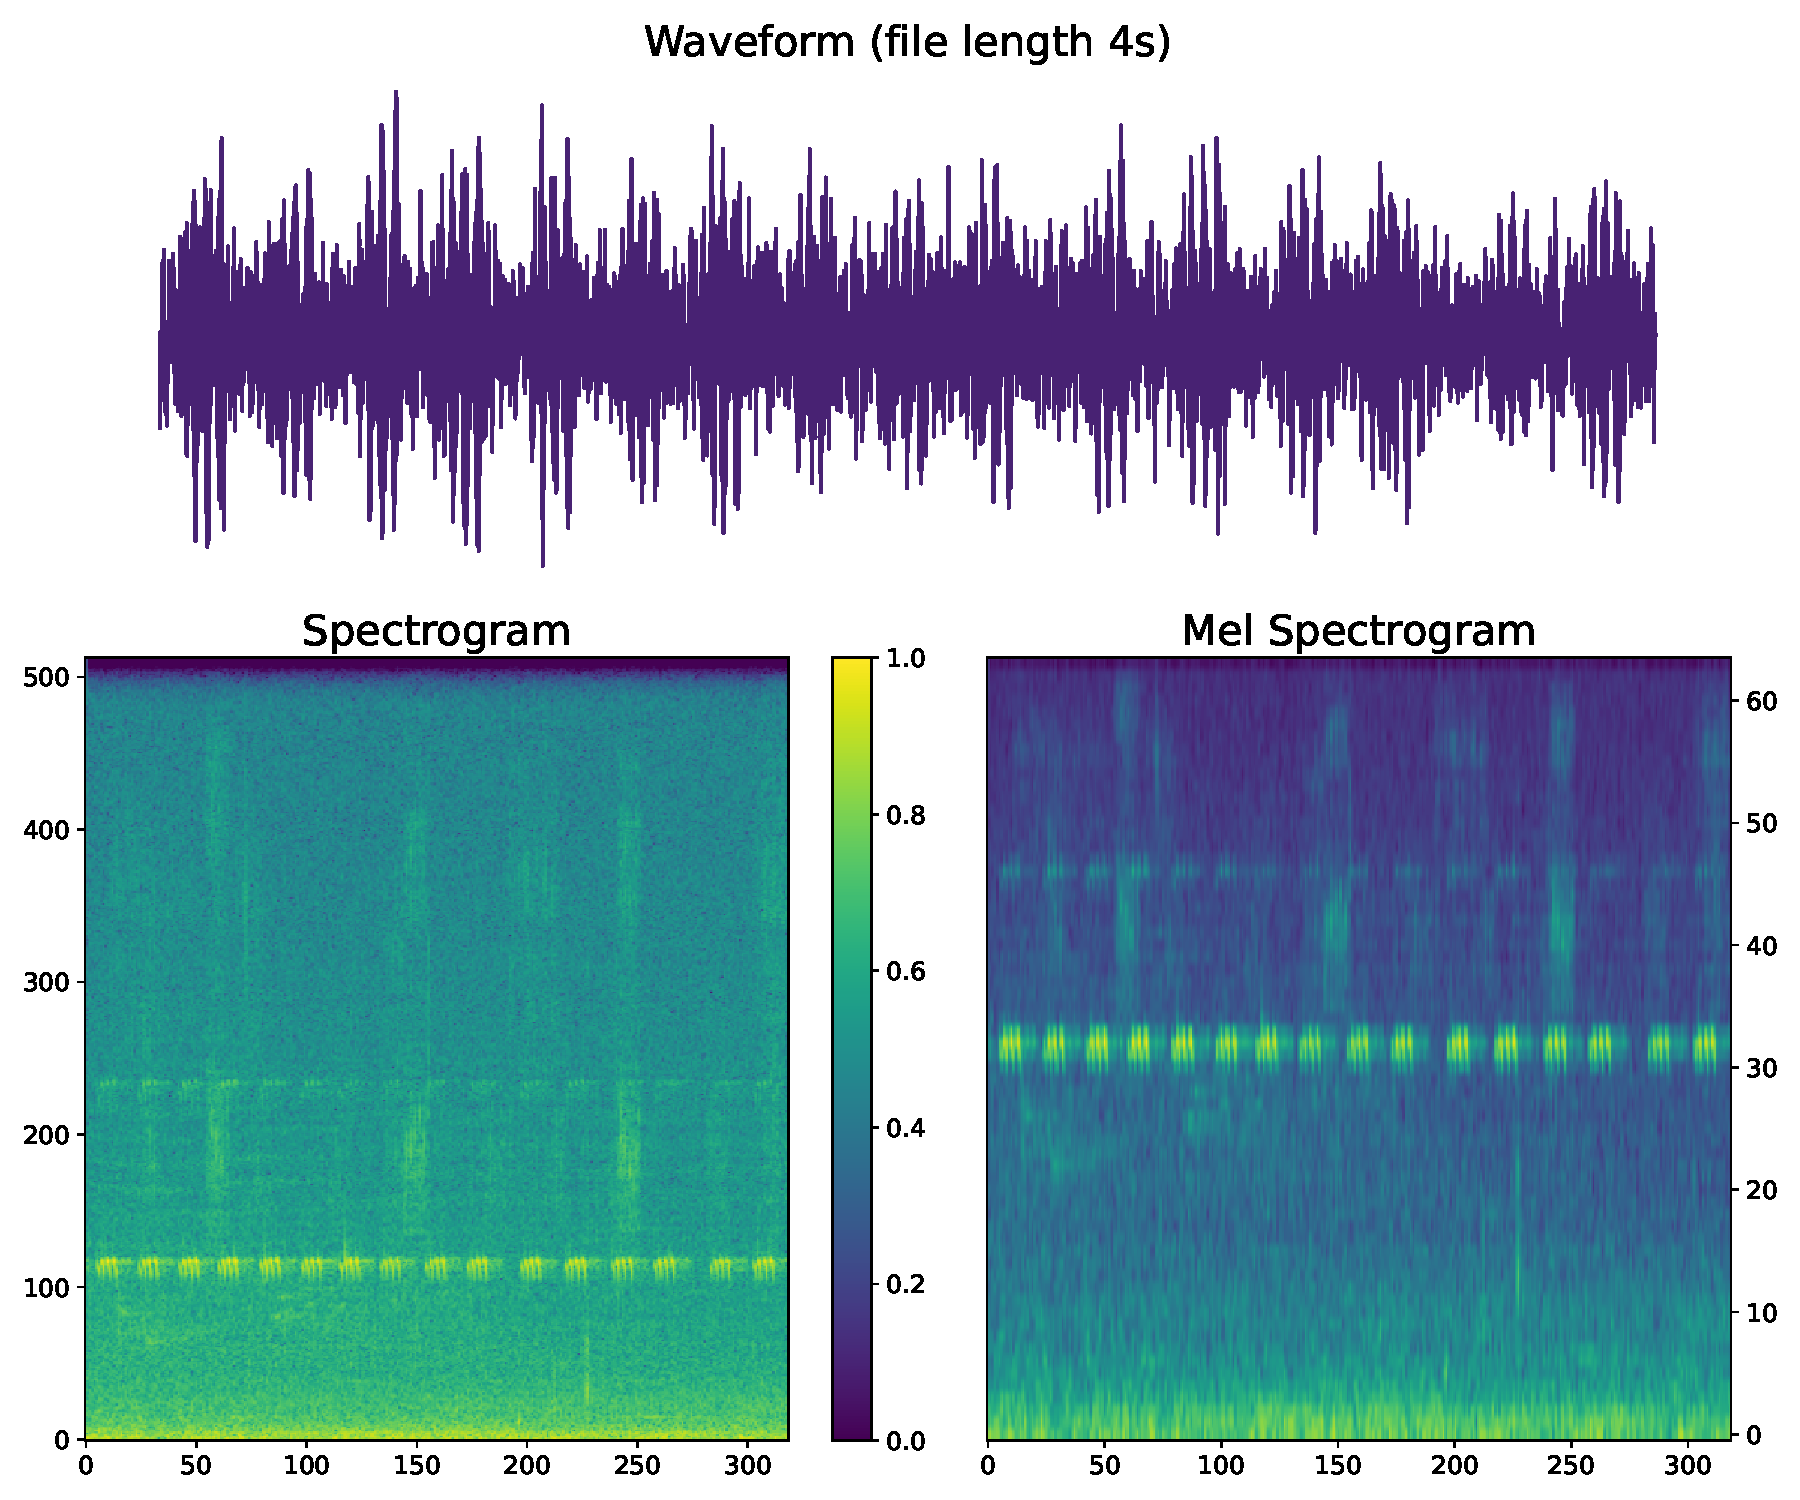
\includegraphics{figures/compare_spectrogram.pdf}
\caption{Visualization of the two transformations of the audio signal.}
\label{fig:compare_spectrogram}
\end{figure}

%=====================================%

%==== figure: model_flow_chart ====%
\begin{figure}[h]
    \centering
    \captionsetup{width=.9\linewidth}
    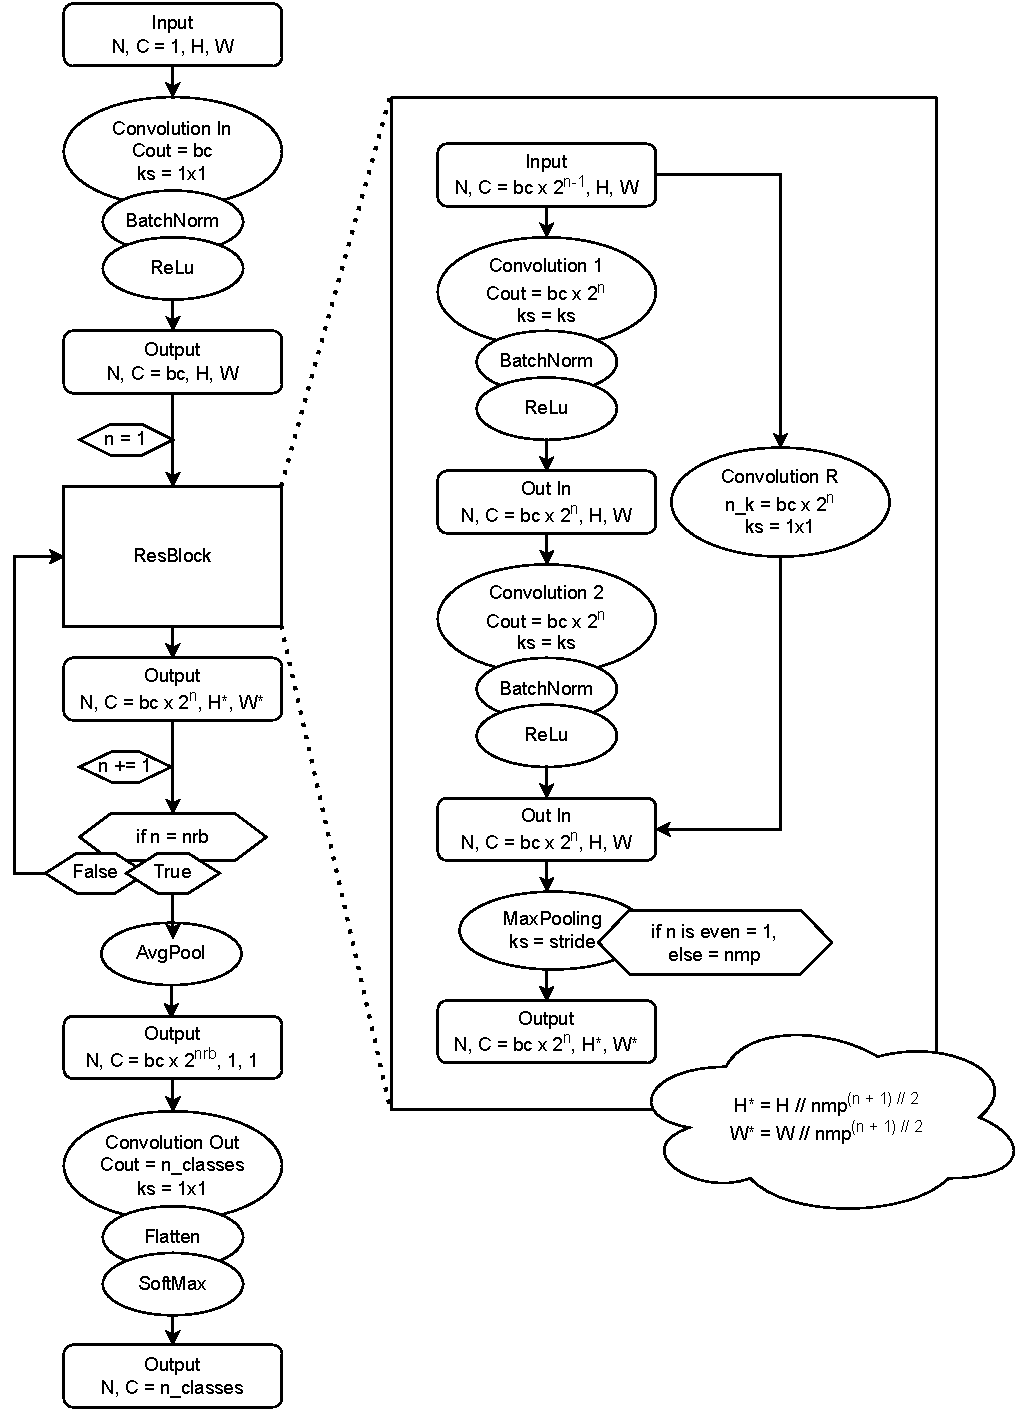
\includegraphics[width=1\textwidth]{figures/model_flow_chart.pdf}
    \caption{
        Flow chart illustrating the models architecture. N: elements in batch, C: channels, H: height, W: width,
        Cout: output channels, ks: kernel size, bc: base channels, nrb: number of residual blocks,
        n\_classes: number of classes, nmp: parameter for max pooling
        }
    \label{fig:model_flow_chart}
\end{figure}
%==================================%